\documentclass[12pt]{article}
% \usepackage[top=1in,left=1in, right = 1in, footskip=1in]{geometry}
\usepackage[top=1in,footskip=1in]{geometry}

\usepackage{graphicx}
\usepackage{xspace}
%\usepackage{adjustbox}

\usepackage{grffile}

\newcommand{\comment}{\showcomment}
%% \newcommand{\comment}{\nocomment}

\newcommand{\showcomment}[3]{\textcolor{#1}{\textbf{[#2: }\textsl{#3}\textbf{]}}}
\newcommand{\nocomment}[3]{}

\newcommand{\jd}[1]{\comment{cyan}{JD}{#1}}
\newcommand{\swp}[1]{\comment{magenta}{SWP}{#1}}
\newcommand{\bmb}[1]{\comment{blue}{BMB}{#1}}
\newcommand{\djde}[1]{\comment{red}{DJDE}{#1}}

\newcommand{\eref}[1]{Eq.~(\ref{eq:#1})}
\newcommand{\fref}[1]{Fig.~\ref{fig:#1}}
\newcommand{\Fref}[1]{Fig.~\ref{fig:#1}}
\newcommand{\sref}[1]{Sec.~\ref{#1}}
\newcommand{\frange}[2]{Fig.~\ref{fig:#1}--\ref{fig:#2}}
\newcommand{\tref}[1]{Table~\ref{tab:#1}}
\newcommand{\tlab}[1]{\label{tab:#1}}
\newcommand{\seminar}{SE\mbox{$^m$}I\mbox{$^n$}R}

\usepackage{amsthm}
\usepackage{amsmath}
\usepackage{amssymb}
\usepackage{amsfonts}
\usepackage[utf8]{inputenc} % make sure fancy dashes etc. don't get dropped

\usepackage{lineno}
\linenumbers

\usepackage[pdfencoding=auto, psdextra]{hyperref}

\usepackage{natbib}
\bibliographystyle{unsrt}
\date{\today}

\usepackage{xspace}
\newcommand*{\ie}{i.e.\@\xspace}

\usepackage{color}

\newcommand{\Rx}[1]{\ensuremath{{\mathcal R}_{#1}}\xspace} 
\newcommand{\RR}{\ensuremath{{\mathcal R}}\xspace}
\newcommand{\Rres}{\Rx{\mathrm{res}}}
\newcommand{\Rinv}{\Rx{\mathrm{inv}}}
\newcommand{\Rhat}{\ensuremath{{\hat\RR}}}
\newcommand{\Rt}{\ensuremath{{\mathcal R}(t)}\xspace}
\newcommand{\tsub}[2]{#1_{{\textrm{\tiny #2}}}}
\newcommand{\dd}[1]{\ensuremath{\, \mathrm{d}#1}}
\newcommand{\dtau}{\dd{\tau}}
\newcommand{\dx}{\dd{x}}
\newcommand{\dsigma}{\dd{\sigma}}

\newcommand{\rx}[1]{\ensuremath{{r}_{#1}}\xspace} 
\newcommand{\rres}{\rx{\mathrm{res}}}
\newcommand{\rinv}{\rx{\mathrm{inv}}}

\newcommand{\psymp}{\ensuremath{p}} %% primary symptom time
\newcommand{\ssymp}{\ensuremath{s}} %% secondary symptom time
\newcommand{\pinf}{\ensuremath{\alpha_1}} %% primary infection time
\newcommand{\sinf}{\ensuremath{\alpha_2}} %% secondary infection time

\newcommand{\psize}{{\mathcal P}} %% primary cohort size
\newcommand{\ssize}{{\mathcal S}} %% secondary cohort size

\newcommand{\gtime}{\tau_{\rm g}} %% generation interval
\newcommand{\gdist}{g} %% generation-interval distribution
\newcommand{\idist}{\ell} %% incubation-period distribution

\newcommand{\total}{{\mathcal T}} %% total number of serial intervals

\usepackage{lettrine}

\newcommand{\dropcapfont}{\fontfamily{lmss}\bfseries\fontsize{26pt}{28pt}\selectfont}
\newcommand{\dropcap}[1]{\lettrine[lines=2,lraise=0.05,findent=0.1em, nindent=0em]{{\dropcapfont{#1}}}{}}

\begin{document}

\begin{flushleft}{
	\Large
	\textbf\newline{
		Intermediate levels of symptomaticity can lead to the worst population-level outcomes
	}
}
\newline
\\
Joshua Weitz\textsuperscript{1,2,3},
Sang Woo Park\textsuperscript{4},
Jonathan Dushoff\textsuperscript{5,6,7}
\\
\bigskip
\textbf{1} School of Biological Sciences, Georgia Institute of Technology, Atlanta, GA, USA
\\
\textbf{2} School of Physics, Georgia Institute of Technology, Atlanta, GA, USA
\\
\textbf{3} Institut de Biologie, \'{E}cole Normale Sup\'{e}rieure, Paris, France
\\
\textbf{4} Department of Ecology and Evolutionary Biology, Princeton University, Princeton, NJ, USA
\\
\textbf{5} Department of Biology, McMaster University, Hamilton, ON, Canada
\\
\textbf{6} Department of Mathematics and Statistics, McMaster University, Hamilton, ON, Canada
\\
\textbf{7} M.\,G.\,DeGroote Institute for Infectious Disease Research, McMaster University, Hamilton, ON, Canada
\\
\bigskip

\bigskip
\end{flushleft}

SARS-CoV-2 has had devastating effects at the population level even as individuals have experienced highly disparate infection outcomes.
Notably, many individuals have mild or even asymptomatic cases making it harder to estimate the magnitude of spread and fatality rate. 
The documented case-fatality rate (CFR) at the population level varies with population, testing infrastructure, and case definitions, typically between 1\%--4\% \citep{rajgor2020many,VERITY2020669,yang2020early}.
But, many infections are never documented. 
The infection fatality rate (IFR), which takes undocumented infections into account, has been estimated to be closer to 0.5\%--1\% for demographics similar to that of the United States \citep{levin2020assessing}. 
This means that more than 99\% of individuals infected with COVID-19 will survive. 
Moreover, at least half of the infections are sufficiently mild that they could be classified as subclinical and even asymptomatic. 
Yet, asymptomatically infected individuals can still transmit to others. 
Hence, asymptomatic infections can be a double-edged sword.
On the one hand, an asymptomatic infection means that the individual infected avoids hospitalization and fatality. 
On the other hand, asymptomatic infections are less likely to be detected \citep{fraser2004factors}, and are may therefore be more likely to infect others, since precautions are less likely to be taken.
This means that the prevalence of asymptomatic infections can paradoxically make population-level outcomes worse than if SARS-CoV-2 was more dangerous at the individual level.

To explore this idea, we propose a simple epidemic model,
in which infected individuals can be asymptomatically or symptomatically infected, with probabilities $p$ and $1-p$, respectively (\fref{base}).  
Asymptomatically infected individuals always recover, whereas a fraction $f$ of symptomatically infected individuals die.
Asymptomatically and symptomatically infected individuals can also have different infection characteristics, including their transmission rates ($\beta_a$ and $\beta_s$) and recovery rates ($\gamma_a$ and $\gamma_s$).
Our key assumption is symptomatically infected individuals take precautions (e.g., reducing contacts or mask-wearing) and therefore reduce their transmission rate by a fraction $\delta$;
we note that the parameter $\delta$ may also capture intervention measures that target symptomatically infected individuals, such as symptom-based isolation. 
As our nominal parameters, we assume lower transmission rates for asymptomatically infected individuals ($\beta_a = 0.75 \beta_s$) and equal recovery rates ($\gamma_a = \gamma_s$).
We assume that asymptomatic individuals do not die, and evaluate the effects of changing the asymptomatic proportion $p$ while holding the fatality rate for \emph{symptomatic} cases, $f$, constant (the IFR $(1-p)f$ thus decreases as $p$ increases).

\begin{figure}[!ht]
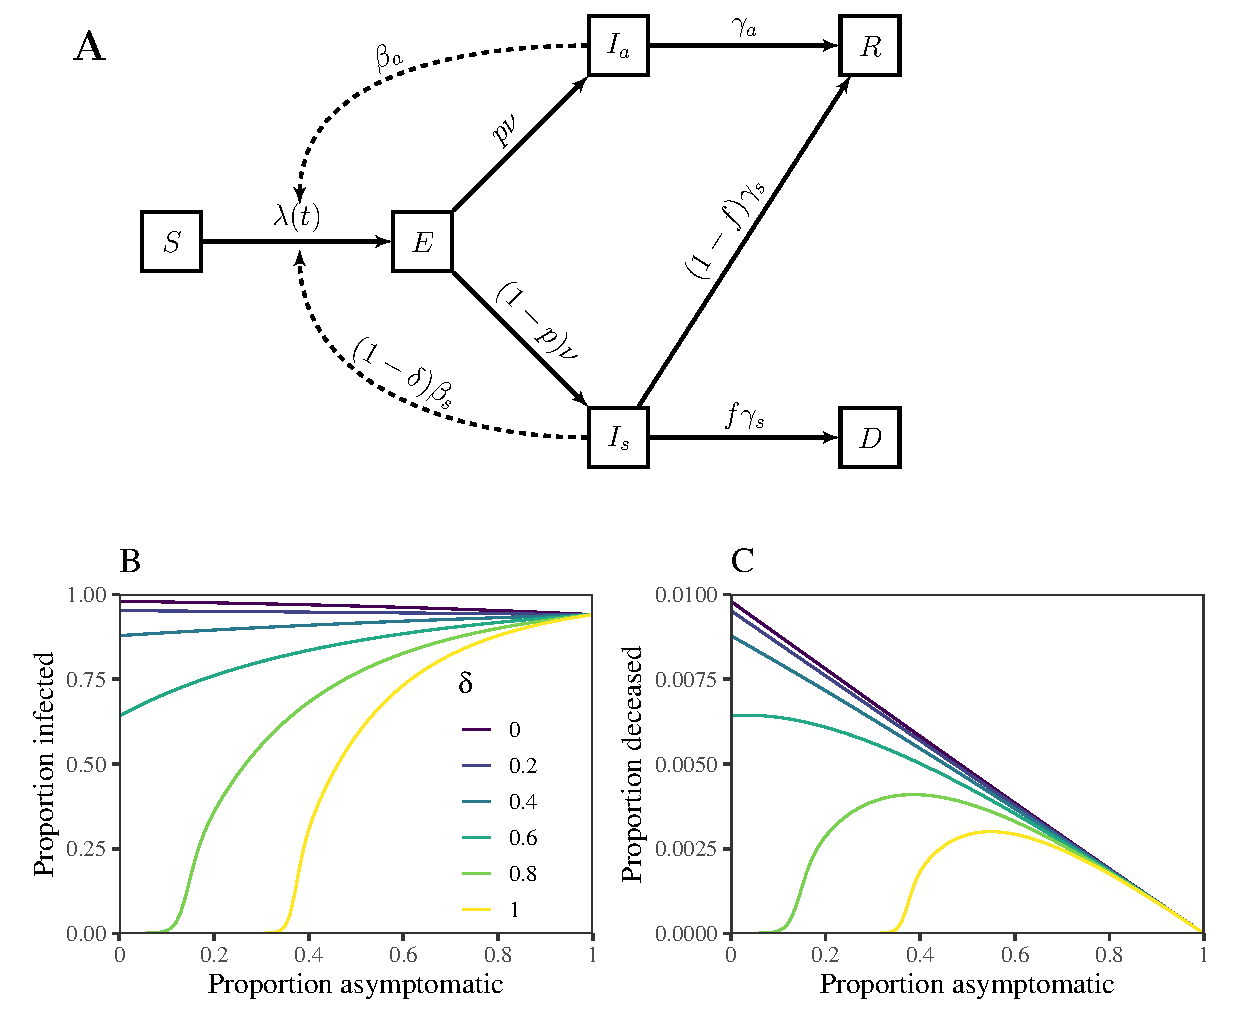
\includegraphics[width=\textwidth]{diagram_base.pdf}
\caption{
\textbf{Schematic diagram and simulations of a model with asymptomatic transmission and symptom-responsive transmission reduction.}
(Left) $S$ represents suceptible individuals; $E$ represents exposed individuals; $I_a$ represents asymptomatically infected individuals; $I_s$ represents symptomatically infected individuals; $R$ represents recovered individuals; and $D$ represents deceased individuals. See Methods for model details.
(Middle) Total infections as a function of the proportion of asymptomatic infections $p$ across a wide range scenarios for $\delta$.
(Right) Total deaths as a function of the proportion of asymptomatic infections $p$ across a wide range scenarios for $\delta$.
We simulate the model for 365 days, assuming $\beta_s = 4/5/\mathrm{day}$, $\beta_a = 0.75 \beta_s$, $\mu=1/2/\mathrm{day}$, $\gamma_s=\gamma_a=1/5/\mathrm{day}$, and $f=0.01$.
We assume that $10^{-4}$ proportion of individuals are initially infected.
}
\label{fig:base}
\end{figure}

\fref{base} evaluates epidemic outcomes using epidemiological parameters similar to that of the originating strain of SARS-CoV-2, without any mitigation other than that individuals who are symptomatic reduce their transmission rate by $\delta$. 
In the absence of the behavioral effect ($\delta=0$), the final size decreases with the asymptomatic proportion $p$ because more symptomatic infections leads to a higher basic reproductin number:
\begin{equation}
\RR_0 = (1-p) (1-\delta) \RR_s + p \RR_a,
\end{equation}
where $\RR_s = \beta_s/\gamma_s$ and $\RR_a = \beta_a/\gamma_a$ represent the reproduction numbers of asymptomatic and symptomatic individuals.
This relationship changes as $\delta$ increases.
In particular, when $\delta > 1-\RR_a/\RR_s$ (in our case, $\delta > 0.25)$, the basic reproduction number increases with $p$ because the behavioral effect causes the effective symptomatic transmission rate to be lower than that that of asymptomatic individuals;
therefore, the number of infections increases with $p$.
For even higher values of $\delta$, we find that there is a critical level of asymptomatic propotion, $p_c$:
\begin{equation}
    p_c = \frac{1 - (1-\delta) \RR_s}{\RR_a - (1-\delta) \RR_s}
\end{equation}
such that $p>p_c$ is required for an outbreak. 
In the limit that $\delta=1$ (i.e., when symptomatically individuals does not transmit at all), then $p_c=1/\RR_a$.

More intricate patterns emerge for fatalities.
When $\delta = 0$, total fataities decrease with $p$ because IFR ($(1-p)f$) decreases.
In contrast, for high values of $\delta$, the peak fatality occurs at intermediate levels of asymptomatic spread:
although less individuals die per infection for higher values of $p$, the increase in total infections also leads to an increase in total fatalities.

High values of $\delta$ required for the nonlinear effects of asymptomaticity on deaths may seem unrealistic---in practice, $\delta$ cannot be greater than the amouont of post-symptomatic transmission.
While several studies have estimated the proportion of pre-symptomatic transmission to be around 30\%--60\% for the SARS-CoV-2 wildtype strain, many of them were likely subject to intervention and behavioral effects already as they were conducted after SARS-CoV-2 awareness became widespread \citep{he2020temporal}.
Instead, \cite{sender2021unmitigated} recently showed that the proportion of pre-symptomatic transmission can be as low as 20\% (95\%CI: 6\%--32\%) in the absence of intervention measures;
while this study provides indirect support for the feasibility of high $\delta$ values, it is still uncertain whether similar effects can be found in more realistic settings.

We therefore consider a series of mathematical models with increasing complexities to answer a more general question:
does intermediate amount of subclinical transmission lead to peak fatalities?


In Supplementary Figure S1, we therefore consider a more realistic model which includes a presymptomatic stage before asymptomatic and symptomatic stages; and we assume that the behavioral effect


We then extend the model to understand the impact of immunity on the severity of the disease by dividing the population into two groups: immunologically naive and protected.
The dynamics of immunologically naive individuals are equivalent to our original model (\fref{base}).
The dynamics of protected individuals include three additional parameters, which characterize the amount of protection against infection $\epsilon_i$, symptoms $\epsilon_s$, and deaths $\epsilon_d$ (\fref{immune}).
For simplicity, we assume that the population is exactly split in half (50\% naive and 50\% protected) and mixes homogeneously; we do not consider the effect of immunity on transmission.
We assume a relatively strong behaviroal effect $\delta=0.8$ for illustration.

\begin{figure}[!ht]
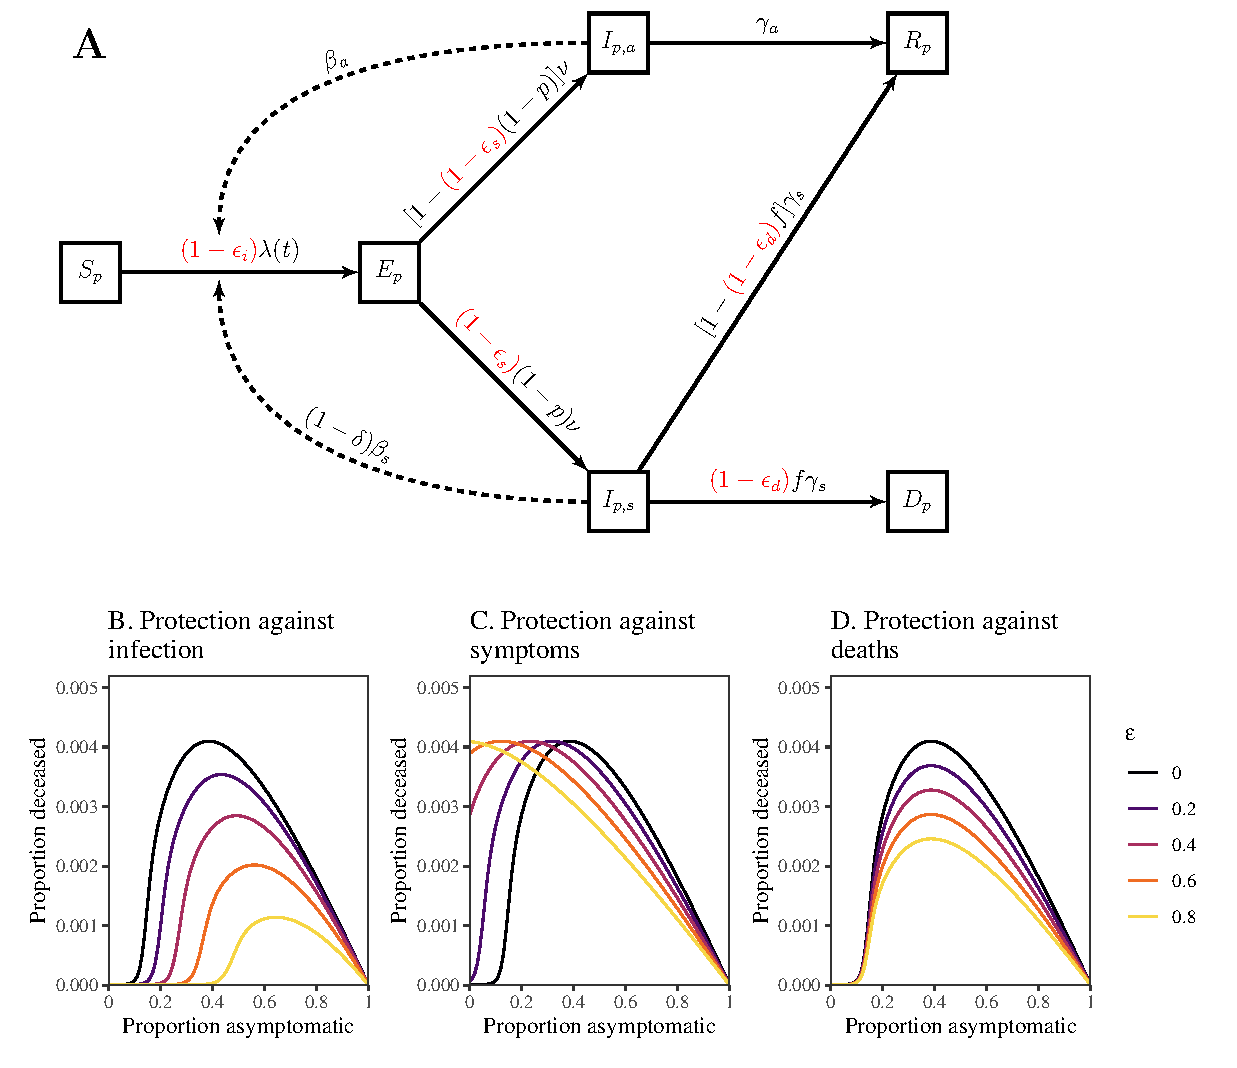
\includegraphics[width=\textwidth]{diagram_immune.pdf}
\caption{
\textbf{Schematic diagram and simulations of a model with symptom-responsive transmission reduction and immunity.}
(Top) The subscript $p$ represents protected individuals. 
Immunity may provide protection against infection, symptoms, or deaths.
The dynamics of immunologically naive individuals are described in (\fref{base}).
(Bottom) Total deaths as a function of the proportion of asymptomatic infections $p$ across a wide range scenarios for protection against infection $\epsilon_i$, symptoms $\epsilon_s$, and deaths $\epsilon_d$.
We simulate the model for 365 days, assuming $\beta_s = 4/5/\mathrm{day}$, $\beta_a = 0.75 \beta_s$, $\mu=1/2/\mathrm{day}$, $\gamma_s=\gamma_a=1/5/\mathrm{day}$, $f=0.01$, and $\delta=0.8$.
We assume that $10^{-4}$ proportion of individuals are initially infected.
}
\label{fig:immune}
\end{figure}

The impact of protection against infection $\epsilon_i$ is analogous to changing $\RR_0$ in the original model: as immunity provides stronger protection against infection (higher $\epsilon_i$), the number of deaths decreases and a higher asymptomatic fraction $p$ is required for the infection to spread (\fref{immunity}A).
We note that protection against infection scales the fatality curve nonlinearly, reflecting the nonlinear relationship between $\RR_0$ and the final size.
The impact of protection against symptoms $\epsilon_s$ is exactly equivalent to changing fraction asymptomatic $p$ for the protected population:
the fatality curves move left as we increase the degree of protection $\epsilon_s$ (\fref{immunity}B).
Therefore, for low values of $p$, protection against symptoms can inadvertently increase the total number of fatalities at the population level by increasing the proportion (and number) of asymptomatically infected individuals, who can readily transmit infections to other individuals.
This also means that the critical level of asymptomatic propotion decreases, allowing more dangeous infections (with lower $p$) to invade, which would not have been able to spread in an otherwise immunologically naive population.
Protection against deaths $\epsilon_d$ directly modulates the fatality rate for symptomatic cases and therefore linearly scales the fatality curves (\fref{immunity}C).

\begin{figure}[!ht]
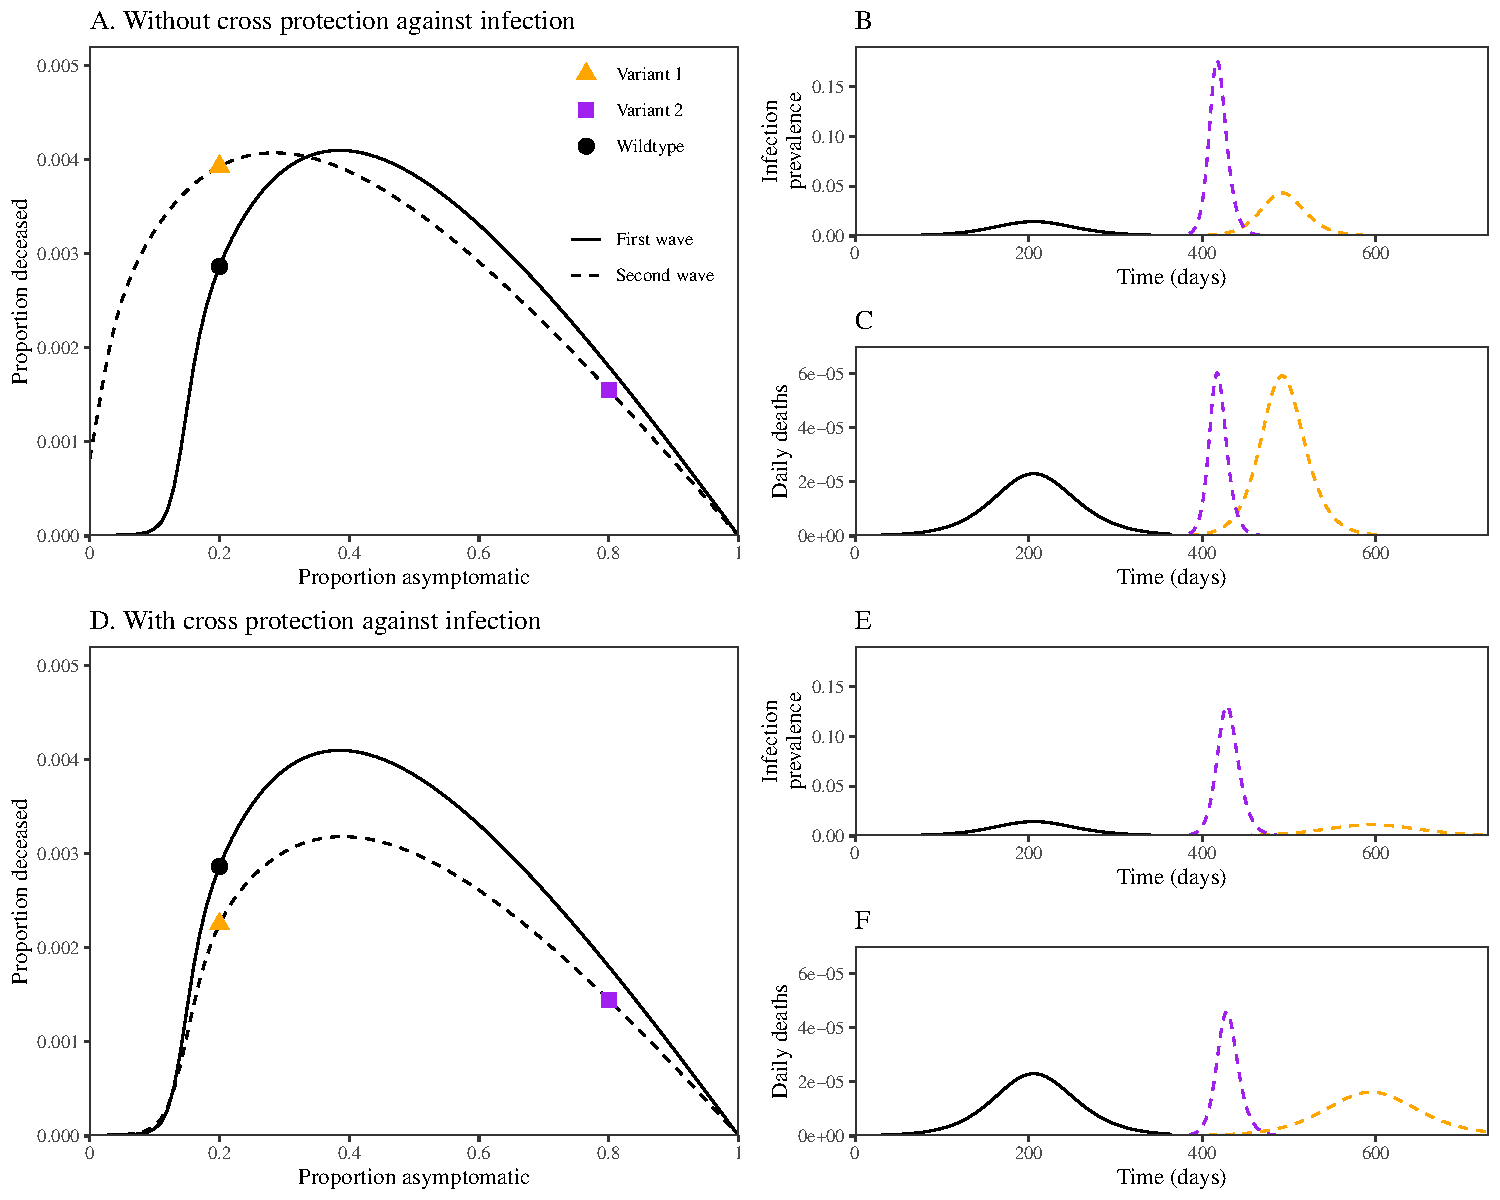
\includegraphics[width=\textwidth]{figure_variant.ggp.pdf}
\caption{
\textbf{Dynamics of invading variants under symptom-responsive transmission reduction and immunity.}
(Top) The subscript $p$ represents protected individuals. 
Immunity may provide protection against infection, symptoms, or deaths.
The dynamics of immunologically naive individuals are described in (\fref{base}).
(Bottom) Total deaths as a function of the proportion of asymptomatic infections $p$ across a wide range scenarios for protection against infection $\epsilon_i$, symptoms $\epsilon_s$, and deaths $\epsilon_d$.
We simulate the model for 365 days, assuming $\beta_s = 4/5/\mathrm{day}$, $\beta_a = 0.75 \beta_s$, $\mu=1/2/\mathrm{day}$, $\gamma_s=\gamma_a=1/5/\mathrm{day}$, $f=0.01$, and $\delta=0.8$ for illustration.
We assume that $10^{-4}$ proportion of individuals are initially infected.
}
\label{fig:variant}
\end{figure}

Finally, we use our framework to understand the impact of behavioral effects on invading variants (\fref{variant}).
In doing so, we first simulate the dynamics of a resident variant for 1 year using our base model (\fref{base}).
We then simulate a new variant invading a partially immune population using our extended model (\fref{immune}), where the immunity is solely derived from natural infections caused by the resident variant.
We consider two types of variants (which are simulated separately): one with the same severity $p$ (orange) and a milder one with higher $p$ (purple).

First, we consider a scenario in which immunity only provides protection against symptoms, $\epsilon_s = 0.4$ (\fref{variant}A--C).
In this case, protection against symptoms allows new variants to spread faster, resulting in larger outbreaks (\fref{variant}B).
Although, a milder (purple) variant exhibits a faster epidemic growth rate and reaches a higher peak (\fref{variant}B), it reaches similar peak fatality as the more severe (orange) variant (\fref{variant}C).
The asymptomaticity--fatality curve provides additional insight (\fref{variant}A): even though a milder, invading variant (purple square) gives higher peak fatality than the original, resident variant (black circle), it leads to lower fatalities overall because deaths are concentrated over a shorter period of time.
In general, invading variants with similar asymptomaticity $p$ will spread better and result in worse population-level outcomes if immunity (either from vaccination or natural infection) provides protection against symptoms, given that asymptomatically infected individuals can transmit better than symptomatically infected individuals (due to either behavioral and intervention effects).

Next, we consider a more realistic scenario in which immunity provides protection against symptoms, $\epsilon_s = 0.4$, and infection, $\epsilon_i = 0.4$ (\fref{variant}D--F).
In this case, cross protection against infection has a disproportionately larger effect on the more severe (orange) variant, causing its peak infection prevalence (\fref{variant}E) and fatality (\fref{variant}F) to be lower than that of the original, resident variant.
Across a wide range of asymptomatic proportion $p$, we find that this immunity profile is sufficient to prevent worse outcomes at the population level.

In summary, using a simplified model we have shown that asymptomatic infections can represent a double-edge sword insofar as they represent a better outcome for some individuals but a mechanism for onwards transmission that leads to a worse outcome for the population as a whole.
Extending our framework further shows that the immunity profile plays a critical role in determining the dynamics of future variants:
while protection against symptoms prevent diseases at the individual level, it can inadvertently lead to more infections, and potentially deaths, at the population level.
For example, milder variants can result in even faster epidemic growth rates and larger outbreaks, even though it can lead to less fatalities if the variant is sufficiently mild.

Our simulatons of invading variants resemble the dynamics of the SARS-CoV-2 Omicron variant.
Despite moderate levels of vaccine effectivenss against symptomatic and severe cases caused by the Omicron variant, especially after booster shots \citep{andres2022omicron}, both vaccine- and infection-derived immunity has provided limited protection against infections \citep{pearson2021omicron}.
Its immune evasive property allowed the Omicron variant to cause more infections in South Africa than previous variants \citep{sun2022omicron};
therefore, even though the Omicron variant has been estimated to be milder \citep{MENNI20221618,ulloa2022estimates}, the number of hospitalizations and deaths caused by the Omicron variant have remained high \citep{Iacobuccio254,faust2022omicron,sigal2022estimating}.

There are several limitations to our analysis.
First of all, behavioral and intervention effects must 

SARS-CoV-2 has proven hard to control in large part because transmission is often decoupled from symptoms. 
Although mitigation efforts have often prioritized responding to symptoms---including symptom-based testing, fever checks, mask-wearing for infectious individuals---a different approach that strives to reduce the chance of asymptomatic transmission while increasing treatment of symptomatically infected individuals could both reduce infection risk at the source and in the event that individuals are at risk for severe outcomes.
As more variants continue to emerge, updating vaccines to prevent infections, and not just diseases, is 



\section*{Methods}
\label{sec.methods}
The model dynamics are as follows
\begin{eqnarray}
\dot{S}=\beta_a S I_a -(1-\delta) \beta_s S I_s \\
\dot{E} = \beta_a S I_a + (1-\delta) \beta_s S I_s - \mu E\\
\dot{I}_a = p \mu E - \gamma_a I_a\\
\dot{I}_s = (1-p) \mu E -\gamma_s I_s\\
\dot{R} = \gamma_a I_a + (1-f) \gamma_s I_s \\
\dot{D} = f \gamma_s I_s
\end{eqnarray}
where the transmission rate $\beta$ and recover rate $\gamma$ can be potentially differ
between asymptomatic and symptomatically infected individuals.  Here, $\delta$ denotes the reduction in transmissability due to responsive measures taken by symptomatically infected indivivduals. Note that the SEIR model framework does not impact final size outcomes, so for convenience, all final size simulations ignore the $E$ class.

\bibliography{main}

\end{document}
